% mit_slideroom_bridge.tex
% Compile with: pdflatex --shell-escape mit_slideroom_bridge.tex  (run twice for refs)

\documentclass[11pt]{article}

\usepackage[utf8]{inputenc}
\usepackage[T1]{fontenc}
\usepackage{lmodern}
\usepackage{graphicx}
\usepackage{xcolor}
\makeatletter
\providecommand\IfPDFManagementActiveF[1]{#1}
\makeatother

\usepackage{svg}
\svgsetup{inkscapepath=photos/}
\usepackage{float}
\usepackage[hidelinks]{hyperref}
\usepackage{geometry}
\usepackage{caption}
\usepackage{enumitem}
\usepackage{microtype}
\usepackage[normalem]{ulem}
\usepackage{booktabs}
\usepackage{siunitx}
\usepackage{amsmath}

\geometry{margin=1in}
\setlist[itemize]{leftmargin=*, itemsep=2pt, topsep=2pt}
\setlist[enumerate]{leftmargin=*, itemsep=2pt, topsep=2pt}

\graphicspath{{photos/}}

\newcommand{\fullwidthfig}[3]{%
\begin{figure}[H]
  \centering
  \includegraphics[width=\linewidth]{#1}
  \caption{#2}
  \label{#3}
\end{figure}
}

\newcommand{\fullwidthsvg}[3]{%
\begin{figure}[H]
  \centering
  \includesvg[width=\linewidth]{#1}
  \caption{#2}
  \label{#3}
\end{figure}
}

\newcommand{\TODO}[1]{\textbf{\textcolor{red}{#1}}}

\definecolor{svgDarkBg}{HTML}{121212}
\definecolor{svgDarkFg}{HTML}{F5F7FA}
\newcommand{\darkincludesvg}[2][]{%
  \begingroup
  \setlength{\fboxsep}{6pt}%
  \colorbox{svgDarkBg}{%
    \parbox{\dimexpr\linewidth-2\fboxsep\relax}{%
      \centering
      \color{svgDarkFg}\includesvg[#1]{#2}%
    }%
  }%
  \endgroup
}

\title{\vspace{-1.2em}Differentiable-Physics Truss Optimizer}
\author{Gabriel Jordaan}
\date{}

\begin{document}
\maketitle
\vspace{-0.75em}

% --- Header strip: logo + quick facts ---
\begin{minipage}[t]{0.22\linewidth}
  \vspace{0pt}
  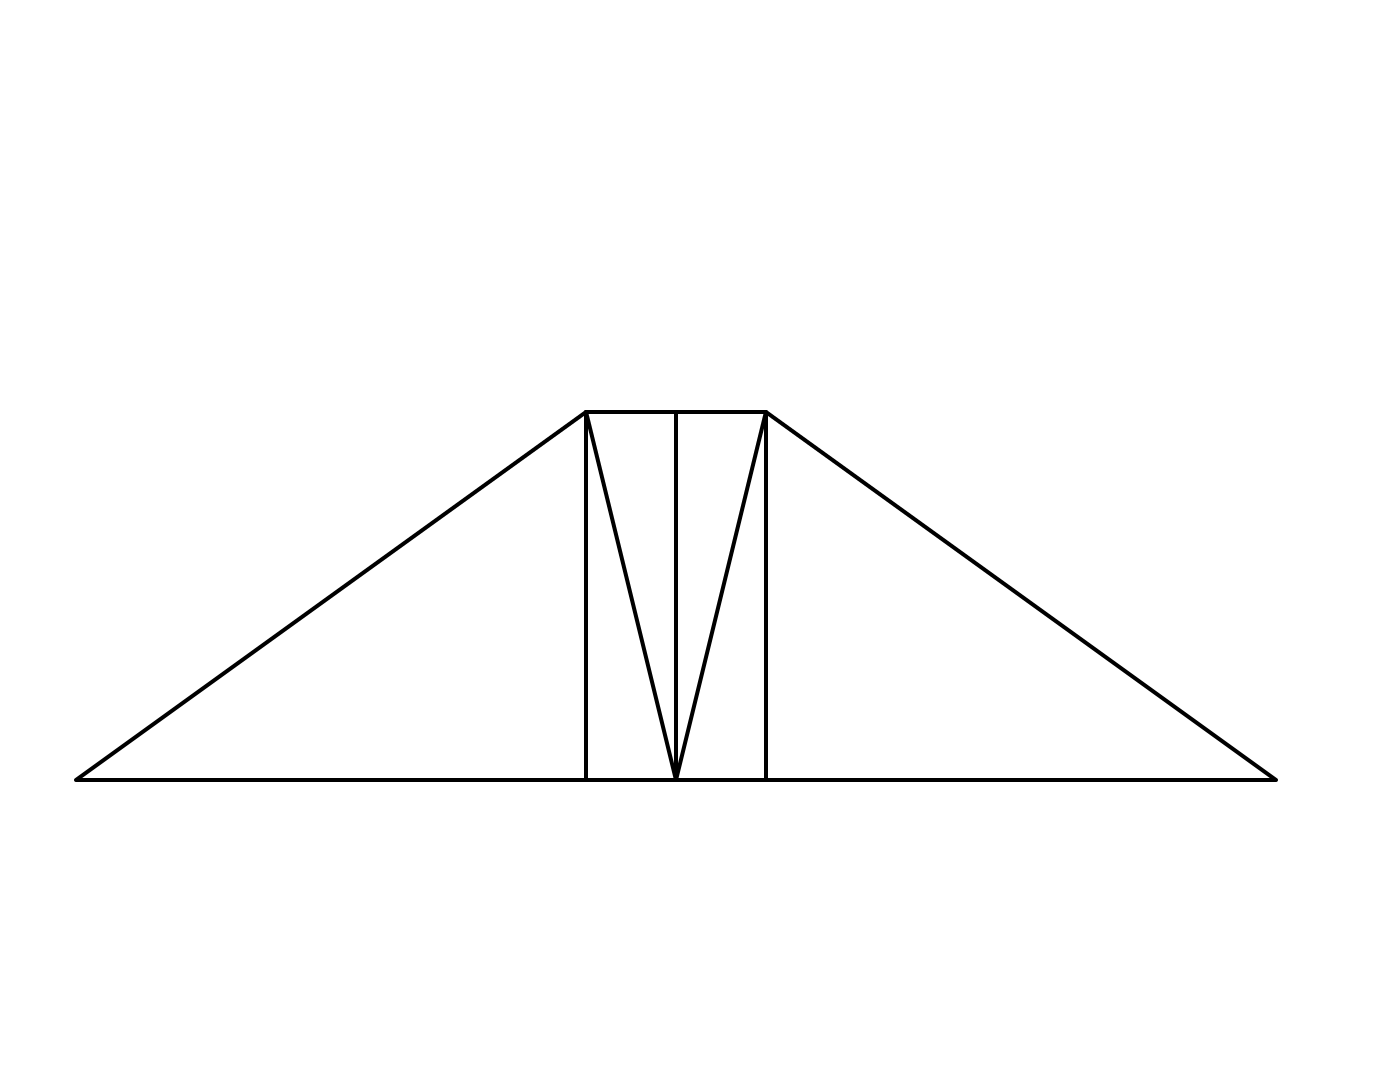
\includegraphics[width=\linewidth]{bridgepic.png}
\end{minipage}\hfill
\begin{minipage}[t]{0.75\linewidth}
  \vspace{0pt}
  \textbf{One-line summary:} This differentiable-physics truss optimizer was developed as a tool for developing the optimal bridge for a second-year statics competition at the University of Nevada, Reno.

  \vspace{0.5em}
  \textbf{GitHub:} \href{https://github.com/ACertainArchangel/truss-optimizer}{https://github.com/ACertainArchangel/truss-optimizer}

\end{minipage}

\vspace{0.8em}
\hrule
\vspace{0.8em}

\noindent
\textbf{Collaborators:} (The other two people on my team in the statics class helped with the assembly of one of the bridges, but I did the second bridge and the software independently.)
\begin{itemize}
  \item Yael Rivas-Ceballos
  \item James Dye
\end{itemize}

\vspace{0.8em}
\hrule
\vspace{0.8em}

% =========================
\section{How Does It Work?}
\subsection{Loss function}
The critical load of the bridge can be modeled as:
\[
  \min_{\substack{\text{failure modes} \\ \text{members}}} \mathbf{F_{cr}}
\]
where $F_{cr}$ is the vector of loads at which a member would fail due to a specific failure mode,
assuming all other members and modes hold. By taking the minimum across all failure modes
and members, we find the load at which the bridge first fails.

As long as the members have a differentiable $F_{cr}$ and we have a differentiable weight
function, we can optimise the critical-load-to-weight ratio using a gradient-based method.
We only need to replace $\min$ with a differentiable approximation:
\[
  \operatorname{softmin}(\mathbf{F_{cr}})
  = \frac{\displaystyle\sum_{i=1}^{n} F_{cr_i}\, e^{-\alpha F_{cr,i}}}
         {\displaystyle\sum_{j=1}^{n} e^{-\alpha F_{cr_j}}},
  \qquad \alpha = 10^6
\]
With $\alpha = 10^6$ (equivalently, temperature $= 10^{-6}$), the differentiable objective
is negligibly different from the true minimum and represents the original objective almost
exactly. The sharp transitions between limiting modes do not cause gradient issues: when
one mode has a higher critical load than others no gradient flows through it, and when one
member is the limiting factor the gradient flows through it normally without amplification. 
The \texttt{torch.min()} function could have been used here, but \texttt{softmin} may improve stability.
This has not been tested yet, but at worst it makes no difference.
\subsection{Optimizer}
In this project, I chose Adam with a learning rate of $0.001$ for its simplicity and
robustness.
\subsection{Extensibility and Focus on Pratt Trusses}
While this framework contains the tools to define other truss types, the main focus of
this project (and the only implemented truss type) is the Pratt truss. Defining a new
truss type requires deriving critical-load and weight calculations for that topology; I
only did so for the Pratt truss because that is what I used for the competition.
\subsection{Modeling failure of any given bridge}
In order to find the critical load of a member, you need functions that describe the
stresses in each member as a function of the applied bridge load. For my calculations, I
assume the force is applied downward equally at the three top nodes: the two where the
inclined members meet the top chord, and one in the middle. This is an approximation of
the hydraulic-press setup used in the competition.

Once you have the maximum bending moment and axial force in each member as a function of
bridge load, you can compute the critical load for each failure mode. Here are the modes
and equations used (where $a$ maps bridge load to member axial force via $F_\text{axial}
= a \cdot F$, $b$ is the analogous moment coefficient via $M = b \cdot F$, $c$ is the
distance from the neutral axis to the outer fibre (simply half the thickness for our rectangular case), $I$ is the second moment of area, $A$
is the cross-sectional area, and $K$ is the effective length factor (0.5 in our case because we fix everything in place with copious amounts of epoxy)):

\medskip
\noindent\textbf{Tension members:}
\begin{itemize}
  \item Non-moment carrying:
  \begin{itemize}
    \item Rupture (axial only): $\displaystyle F = \frac{\sigma_t \cdot A}{a}$
  \end{itemize}
  \item Moment carrying:
  \begin{itemize}
    \item Rupture (axial + bending, out of plane MOI has no effect): $\displaystyle F = \frac{\sigma_t}{\dfrac{a}{A} + \dfrac{b \cdot c}{I_{in}}}$
  \end{itemize}
\end{itemize}

\medskip
\noindent\textbf{Compression members:}
\begin{itemize}
  \item Non-moment carrying:
  \begin{itemize}
    \item Crushing (axial only): $\displaystyle F = \frac{\sigma_c \cdot A}{a}$
    \item Euler buckling (axial only): $\displaystyle F = \frac{1}{a} \cdot \frac{\pi^2 E\,I_{min}}{(KL)^2}$
  \end{itemize}
  \item Moment carrying:
  \begin{itemize}
    \item Crushing (axial + bending): $\displaystyle F = \frac{\sigma_c}{\dfrac{a}{A} + \dfrac{b \cdot c}{I_{min}}}$
    \item Euler buckling in plane (axial + bending): $\displaystyle F = \frac{\pi^2 E\,I_{in}\,/\,(KL)^2}{a + b \cdot c \cdot A\,/\,I_{in}}$
    \item Euler buckling out of plane (axial only, moment is in plane): $\displaystyle F = \frac{\pi^2 E\,I_{out}}{a\cdot (KL)^2}$
  \end{itemize}
\end{itemize}

\medskip
\noindent
All seven expressions above are closed form because member forces and moments are both linear in $F$.
In the current v4 implementation, these expressions are evaluated
directly in PyTorch with no numerical methods needed.

These equations assume there are coefficients $a$ and $b$ that map the bridge load to member axial force and bending moment (i.e.\ that the structure is linear), and this assumption holds until yielding begins, at which point it is too late. These models work right up to failure and that is where we need them to work until. For a material with higher ductility than our brittle composite, this would not be the case.
\subsection{Bridge Weight}
To get the weight, we simply sum the volumes of all members, multiply by the material density, and add our estimated fixed cost of fasteners (or glue, in our case). Member volumes are approximated as right rectangular prisms though they are actually right rhombic prisms. We take the volume of a member as $V = L \cdot A$. This discrepancy of volumes is discussed in Section~\ref{sec:challenges}, and it is not significant, because it only affects the ends, which also have epoxy on them that slightly counteracts the missing volume.

% \fullwidthfig{image.jpg}{Caption.}{fig:label}

% =========================
\section{Calculations of relevant quantities for the Pratt Truss (\texttt{PrattV1})}
All we need now are the values of $a$, $b$, $c$, member lengths, and the $I$ in and out of plane for each member in terms of our trainable design parameters (what we can use to get designs), which can be obtained with the following calculations:
\subsection{Pre load path analysis}
\noindent\textbf{Trainable design parameters:}

\begin{table}[H]
\centering
\begin{tabular}{@{}lll@{}}
\toprule
Symbol & Code name \textcolor{white}{007} & Description \\
\midrule
$\theta$                    & \texttt{angle}               & Angle of incline members from horizontal \\
$h$                         & \texttt{height}              & Vertical height of the truss \\
$L$\footnotemark                         & \texttt{span}                & Total horizontal span (fixed by competition rules) \\
\midrule
$t_\text{inc},\,d_\text{inc}$   & \texttt{incline\_thickness, depth}   & Incline member cross-section \\
$t_\text{diag},\,d_\text{diag}$ & \texttt{diagonal\_thickness, depth}  & Diagonal member cross-section \\
$t_\text{mv},\,d_\text{mv}$     & \texttt{mid\_vert\_thickness, depth} & Mid vertical member cross-section \\
$t_\text{sv},\,d_\text{sv}$     & \texttt{side\_vert\_thickness, depth}& Side vertical member cross-section \\
$t_\text{top},\,d_\text{top}$   & \texttt{top\_thickness, depth}       & Top chord cross-section \\
$t_\text{bot},\,d_\text{bot}$   & \texttt{bottom\_thickness, depth}    & Bottom chord cross-section \\
\bottomrule
\end{tabular}
\end{table}
\footnotetext{Length is not a trainable parameter. We just include it in the parameter dictionary for simplicity. Technically you could include it in trainable parameters but it would immediately snap to the lowest possible length, and training length is nonsense.}
\newpage
\noindent\textbf{Derived member lengths (and $\varphi$)} (computed from the trainable parameters each forward pass):

\begin{table}[H]
\centering
\begin{tabular}{@{}lll@{}}
\toprule
Symbol & Expression & Description \\
\midrule
$L_\text{inc}$  & $h / \sin\theta$     & Incline member length \\[4pt]
$L_\text{diag}$ & $h / \cos\varphi$    & Diagonal member length \\[4pt]
$L_\text{top}$  & $L - 2h/\tan\theta$  & Top chord length \\[4pt]
$L_\text{bot}$  & $L$                  & Bottom chord length \\[4pt]
$L_\text{vert}$ & $h$                  & Mid and side vertical length \\
$\varphi$ & $\arctan\!\left(\dfrac{L_\text{top}/2}{h}\right)$ & Diagonal angle from vertical \\[8pt]
\bottomrule
\end{tabular}
\end{table}
 
\fullwidthfig{bridgediagram.png}{Diagram of a Pratt truss with $\theta$ and $\varphi$ angles labeled.}{fig:bridgediagram}

\textbf{Other easy properties:}
\begin{table}[H]
\centering
\begin{tabular}{@{}lll@{}}
\toprule
Symbol & Expression & Description \\
\midrule
$I_{in}$ & $\frac{1}{12} d_\text{member} t_\text{member}^3$ & In-plane member moment of inertia \\
$I_{out}$ & $\frac{1}{12} t_\text{member} d_\text{member}^3$ & Out-of-plane member moment of inertia \\
$A$ & $t_\text{member} \cdot d_\text{member}$ & Cross-sectional area \\
$c$ & $t_\text{member}/2$ & Distance from neutral axis to extreme fiber \\
\bottomrule
\end{tabular}
\end{table}

The reason we have c as the distance from neutral axis to the surface thickness wise (in plane) and not depth wise (out of plane) is because in our model, all bending moments are in the plane before deformation, and all equations with c have to do with bending moments in the plane.
\newline\newline

\subsection{Joint Equilibrium Calculations Used by \texttt{PrattTrussV1}}

Now for the hard-ish part, calculating $a$ and $b$ for each member.
\newline

%%%%%%%%
% BEGIN CALC SECT
%%%%%%%%

We label the nodes of the left half of the symmetric truss as follows (see Figure~\ref{fig:bridgediagram}; we don't have to do the other side because symmetry):
\begin{itemize}
  \item $A$ = bottom-left support (pin, roller, fixed, whatever, it's all downward force so it doesn't matter.)
  \item $B$ = bottom-left panel point (where the left side-vert meets the bottom chord)
  \item $C$ = bottom midpoint (where the two diagonals and mid vert meet the bottom chord)
  \item $D$ = top-left joint (where the left incline meets the top chord)
  \item $E$ = top midpoint (where the mid-vert meets the top chord)
\end{itemize}
By symmetry, the right half is the mirror image. 

\subsubsection{Note on the assumptions we use in modeling the load path}
In our model, the total applied load $F$ is split equally among the three top nodes: $D$, $E$, and the mirror of $D$, $D'$, so each carries $F/3$ downward. As a simplification, we say the verticals carry 1/3 of the load, and that the diagonals "pull the force back up", and back into the inclines. This is not technically exact, but it is a gradient force in the right direction, tests suggest it is very close, and it is meant to be conservative. The inclines in our model are therefore modeled as bearing equivalent vertical stress to the full vertical load, while some passes through verticals and diagonals, which optimize for their own survival.  

\medskip
% ---- Incline Members ----
\subsubsection{Incline Members}

Each support carries half the total load by symmetry, so the vertical reaction at $A$ is $R_A = F/2$ (upward).

Taking vertical equilibrium at A gives
\[
R_A = \frac{F}{2}, \qquad
F_\text{inc}\sin\theta = R_A
\quad\Rightarrow\quad
F_\text{inc} = \frac{F}{2\sin\theta}.
\]
Therefore
\[
\boxed{a_\text{inc} = \frac{1}{2\sin\theta}, \qquad b_\text{inc} = 0.}
\]

% ---- Diagonal Members ----
\subsubsection{Diagonal Members}

For the diagonal pair, we use symmetry again, and the previously mentioned assumption that they must bear 1/3 of the load vertically, so:
\[
2F_\text{diag}\cos\varphi = \frac{F}{3}
\quad\Rightarrow\quad
F_\text{diag} = \frac{F}{6\cos\varphi},
\]
so
\[
\boxed{a_\text{diag} = \frac{1}{6\cos\varphi}, \qquad b_\text{diag} = 0.}
\]

% ---- Vertical Members ----
\subsubsection{Vertical Members}

The vertical members are modeled as sharing a total load of $F/3$ in proportion to their
cross-sectional areas (this works because Hooke's constant $K = E \cdot A/L$ and they all have the same $E$ and $L$). Let
\[
A_\text{sv} = t_\text{sv}d_\text{sv}, \qquad A_\text{mv} = t_\text{mv}d_\text{mv}.
\]
Then
\[
F_\text{sv} = \frac{A_\text{sv}}{2A_\text{sv} + A_\text{mv}}\cdot\frac{F}{3}, \qquad
F_\text{mv} = \frac{A_\text{mv}}{2A_\text{sv} + A_\text{mv}}\cdot\frac{F}{3},
\]
which gives
\[
\boxed{a_\text{sv} = \frac{A_\text{sv}}{2A_\text{sv} + A_\text{mv}}\cdot\frac{1}{3}, \qquad
a_\text{mv} = \frac{A_\text{mv}}{2A_\text{sv} + A_\text{mv}}\cdot\frac{1}{3},}
\]
and
\[
\boxed{b_\text{sv} = b_\text{mv} = 0.}
\]

% ---- Bottom Chord ----
\subsubsection{Bottom Chord}

We say the axial force in the bottom chord equals the sum of the horizontal components of the incline and diagonal forces (worst case of force distribution in which the diagonals do not cancel each other out at all in their effect on the bottom chord):
\[
F_\text{bot} = F_\text{inc}\cos\theta + F_\text{diag}\sin\varphi.
\]
Substituting the force expressions for the inclines and diagonals gives
\[
\boxed{a_\text{bot}
= \frac{\cos\theta}{2\sin\theta} + \frac{\sin\varphi}{6\cos\varphi}.}
\]

Now, we know the maximal moment in the bottom chord will be at the midpoint, and we take the distance $\overline{BC}$ as the lever arm for the forces exerted by the side-vertical members.
\[
\ell = \overline{BC} = \frac{L_\text{top}}{2} = \frac{L}{2} - \frac{h}{\tan\theta}.
\]
Using the side-vertical force as the transverse load on the half-span of the chord, the
code takes
\[
M_\text{bot} = -F_\text{sv}\ell.
\]
Dividing through by $F$ gives
\[
\boxed{b_\text{bot} = -\frac{A_\text{sv}}{2A_\text{sv} + A_\text{mv}}\cdot\frac{1}{3}
\left(\frac{L}{2} - \frac{h}{\tan\theta}\right).}
\]

% ---- Top Chord ----
\subsubsection{Top Chord}

The axial force in the top chord is the same as the bottom chord:
\[
F_\text{top} = F_\text{inc}\cos\theta + F_\text{diag}\sin\varphi,
\]
so
\[
\boxed{a_\text{top}
= \frac{\cos\theta}{2\sin\theta} + \frac{\sin\varphi}{6\cos\varphi}.}
\]

For the moment coefficient, using the side-vertical force as the transverse load on the half-span:
\[
M_\text{top} = +F_\text{sv}\ell,
\]
which gives
\[
\boxed{b_\text{top} = \frac{A_\text{sv}}{2A_\text{sv} + A_\text{mv}}\cdot\frac{1}{3}
\left(\frac{L}{2} - \frac{h}{\tan\theta}\right).}
\]

Because the hydraulic press actually applies load evenly, the moment here would likely be closer to zero, but again, we make conservative assumptions. Setting this to zero would be safe and I may do that in a future version, for now it is included for consistency (this moment never got close to being the critical mode so we should be fine here in v4.)

\medskip
That is the full set of $a$ and $b$ coefficients used in \texttt{pratt\_v1.py}.

%%%%%%%%
% END CALC SECT
%%%%%%%%
% =========================


\section{Material Models}

For this project, the building material was a balsa wood and epoxy composite: 1/16th inch sheets of balsa laminated together with epoxy. This was to take advantage of the fact that the competition rules said we could laminate as much as we wanted, and the professor thought it was hilarious how far I pushed it. The properties of the composite were estimated using the rule of mixtures, and an efficiency factor $\eta$ of 0.9, under the rule of thumb that you generally lose $\sim$10\% efficiency when laminating like this.
From the datasheets, the properties of the balsa wood and epoxy were obtained, and the composite properties were determined as a simple half and half average, then reduced by 10\%. (E and both sigmas)
% =========================

\section{Why a Pratt Truss?}

A Pratt truss was chosen because balsa wood is especially good in tension, and I originally wanted to take advantage of that. What I did not account for at the time of picking a pratt truss, was that the final laminated composite of 50\% epoxy and 50\% balsa would have roughly the average of their compressive and tensile strengths. Epoxy is much better in compression, and by the time I performed the rule of mixtures and found out a compression heavy bridge would have been better, I had already coded the PrattTrussV1 implementation, and felt I was too low on time to research and implement a new truss type. At least for a pratt truss I know I got an optimal one. A Howe truss would likely have been better, and perhaps I will add one in an update.

% =========================
\section{Core Software Architecture}
\label{sec:build}

The workflow for using this software is relatively simple:

\begin{enumerate}
  \item Create a pratt truss object, initialising with your desired parameters.
  \item Initialise a bridge optimiser object, passing in parameters like learning rate and constraints as well as the bridge you want to optimize.
  \item Call: \texttt{convergence\_plot = optimizer.optimize(your parameters like iterations here)}
  \item Extract the bridge again with \texttt{optimizer.bridge}, and get useful information with \texttt{bridge.visualise()} or \texttt{bridge.generate\_report()}
\end{enumerate}

% \fullwidthfig{image.jpg}{Caption.}{fig:label}

\subsection{Pratt Truss Object}
Contains the tensor parameters that define the truss, methods for getting critical load and weight differentiably, a method for visualising, a method for generating a report, and a method for clamping angle to valid ranges to ensure a minimum top chord length.

% \fullwidthfig{image.jpg}{Caption.}{fig:label}

\subsection{Bridge optimizer Object}

Contains the Adam training loop. On each forward pass it uses the critical load to weight ratio from the bridge, and calls \texttt{.backward()} to get gradients with respect to all trainable cross-section and geometry parameters. Parameters are clamped to be within ranges for the competition each step. Optimizing returns an image of the convergence plot.

% \fullwidthfig{image.jpg}{Caption.}{fig:label}

\subsection{Material Object}

Dataclass containing material properties.

\subsection{Interactions Between Modules}

None of the main modules call on each other and interaction is orchestrated manually so it is sandboxed quite nicely.

% \fullwidthfig{image.jpg}{Caption.}{fig:label}

% =========================
\section{Key Challenges and Solutions}
\label{sec:challenges}

\noindent
\begin{itemize}
  \item The simplification of treating members as rectangular prisms instead of right rhombic prisms introduced some error in volume calculations, but this was small, did not break monotonicity with true volume, and was offset by a little extra fixed cost. 
  \item After constructing the first bridge with my teammates, we left it in a cold garage overnight. We later discovered that this made the epoxy brittle, so I rebuilt it on my own in a warm living room, and exceeded the critical load of the first bridge on test day.
  \item Keeping the bridge geometry within legal bounds (legal as in both allowed in the competition and physically possible) was solved by parameter clamping. It's not the most elegant solution but it seems to work well enough as can be seen on convergence plots.
  \item Clamping causes some training volatility, but this can be worked around by fixing height in place and optimising angle, and then initialising many bridges with different heights and taking the best, since fixing one of height and angle, then training the other solves the volatility issue.
  \item After I tried making an updated force calculation in \texttt{PrattTrussV2} that was meant to be more accurate, the new version ended up being worse than my already accurate model, so I deprecated \texttt{PrattTrussV2}.
\end{itemize}

% =========================
\section{Sources and Citations}

\begin{itemize}
  \item \textbf{AI Disclosure for 4v:} 
    \begin{itemize}
      \item Bridge Optimizer v4, the version presented in this report, uses a small number of PyTorch expressions that were transcribed by AI from my handwritten equations (originally written out with the math module). 
      \item I used a single ChatGPT prompt about the FPDF library API, which is used to generate reports.
      \item In earlier versions (especially v2) Copilot was used for scripting and testing, but none of these scripts or tests are in v4.
      \item Inline autocomplete by Github Copilot was used occasionally for completing variable names, closing brackets, and other such boilerplate I was already typing.
    \end{itemize}
  \item \textbf{Libraries:}
  \begin{itemize}
    \item PyTorch, the backbone of the project
    \item Pillow, used for processing bridge visualisations
    \item FPDF, used to generate reports and bills of materials for the bridges.
    \item Matplotlib, used to plot convergence.
  \end{itemize}
  \item \textbf{Datasheets:}
  \begin{itemize}
    \item Ochroma Group. \textit{Ochroma Balsa Wood Specifications v2}. \\
      \href{https://ochromagroup.com/wp-content/uploads/2025/01/SpecSheets/Ochroma-balsa-wood-specs-v2.pdf}{\uline{CLICK FOR DATASHEET}}
    \item Sakrete. \textit{High Strength Anchoring Epoxy --- Product Data Sheet}. \\
      \href{https://www.sakrete.com/wp-content/uploads/2021/07/High-Strength-Anchoring-Epoxy.pdf}{\uline{CLICK FOR DATASHEET}}
    \item CoreLite Composites. \textit{BALSASUD Core Data Sheet} \\
      \href{https://www.corelitecomposites.com/files/BALSASUD%20Core%20Data%20Sheet.pdf}{\uline{CLICK FOR DATASHEET}}
  \end{itemize}
  \item \textbf{Other:}
  \begin{itemize}
    \item Used Black and isort to format the code.
  \end{itemize}
\end{itemize}

% =========================
\section{Results}

\subsection{What worked well}
\begin{itemize}
  \item Exceeded Spring 2023 and Spring 2024 records for critical load to weight ratio by over 4\%. The highest of these was 1181.49 and my bridge scored 1229.3.
  \item Fast convergence. Leaving it running and saving the best design can push performance a little more once the initial good design is found, though.
  \item Model predicted a critical load of 4302 N; actual critical load was 4025 N, meaning it predicted within a 6.88\% error. Pretty good, considering the simplifications made, like the 50\%/50\% volume fraction, and the approximate nature of the load-sharing assumptions built into \texttt{PrattTrussV1}. If we had been more conservative and taken the efficiency factor (\(\eta\)) of our laminate to be 0.85 (the lower end of the 0.85--0.95 rule of thumb range) instead of 0.9, we would have predicted 4082 N, which is within 1.42\% error.
\end{itemize}

\noindent
\subsection{What I would do differently}
\begin{itemize}
  \item Measure the material properties of the composite used rather than relying on the rule of mixtures and theoretical values from data tables. The model was quite accurate but empirical testing of actual material properties could improve accuracy or validate the physics calculations more rigorously.
  \item Not leave the bridge in the cold garage so I would only have to build one :p
  \item Apply a more structured approach to initialising multiple bridges like a grid search or latin hypercube sampling instead of random initialisation for each instance. That way we could ensure more diverse exploration in less time. (I would write this as a usage of the framework, not into the framework itself.)
  \item Apply a more precise method for estimating the weight of members instead of approximating them as rectangular prisms.
  \item Perhaps try differentiable FEA with a framework like JAX FEM to be even more exact.
  \item The repository contains versions 1--4, but this report focuses on Bridge v4, specifically PrattTrussV1 in Bridge v4. Bridge v4 also has a bridge type called PrattTrussV2, that uses an experimental and more complicated model, but the PrattTrussV1 calculations ended up being superior and PrattTrussV2 has been marked as deprecated (though it is still used as a demonstration in \texttt{bridge\_ensemble.py}). In short, the versioning x development process was an absolute saga and I would keep tighter reins on it if I repeated this project.
\end{itemize}

\subsection{Final Note}
I plan to continue tinkering with this project, but given the performance achieved in the competition, I would definitely call it a minimum viable product at the very least. Making it was a lot of fun, I hope you enjoyed reading about it.
% \fullwidthfig{image.jpg}{Caption.}{fig:label}

\end{document}
